\documentclass{sig-alternate-10pt}

\usepackage{graphics}
\usepackage{epsfig}
\usepackage{color}
\usepackage{hyperref}
\usepackage[usenames,dvipsnames]{xcolor}
\usepackage{url} 
\usepackage{underscore}
\usepackage{caption}
\usepackage{subcaption}
\usepackage{graphicx}
\usepackage{times}

%
% Get rid of excess white space, commands copied from:
% http://www.terminally-incoherent.com/blog/2007/09/19/latex-squeezing-the-vertical-white-space/
%
\usepackage{mdwlist}
\setlength{\voffset}{0.0in}
\setlength{\headsep}{5pt}

\newcommand{\eg}{{\em e.g., }}
\newcommand{\ie}{{\em i.e., }}
\newcommand{\paragraphb}[1]{\vspace{0.03in}\noindent{\bf #1} }
\newcommand{\paragraphe}[1]{\vspace{0.03in}\noindent{\em #1} }
\newcommand{\paragraphbe}[1]{\vspace{0.03in}\noindent{\bf \em #1} }
\newcommand{\comment}[1]{\textcolor{purple}{#1}}
%\newcommand{\sysname}{CommunityGuard }
%\newcommand{\servname}{CommunityOutpost server }
%\newcommand{\servnames}{CommunityOutpost servers }
%\newcommand{\nodename}{CommunityGuardian node }
%\newcommand{\nodenames}{CommunityGuardian nodes }


\title{CommunityGuard: A Crowdsourced Home Cyber-Security System}

\author{Chase E. Stewart, Anne Maria Vasu, Eric Keller \\ 
        \{chase.stewart, anne.vasu, eric.keller\}@colorado.edu}

\begin{document}
\setlength{\pdfpagewidth}{8.5in}
\setlength{\pdfpageheight}{11in}

\thispagestyle{empty}

\maketitle


\begin{abstract}
%Internet vandalism is on the rise. Malware such as Mirai, which enabled the 640 Gbps attack on Dyn DNS servers in October of 2016, are available on the free market along with their source code to exploit pre-identified vulnerable target devices. Target device manufacturers appear more concerned about getting products to market and do not focus on security measures that can prevent such attacks. A common user with little to no idea about Network and Security might be unable to distinguish between personal devices, such as IOT devices, that are secure versus those that can be easily attacked.\\

In this paper, we propose and implement \sysname, a system which comprises of intelligent \nodenames that learn and prevent malicious traffic from coming into and going out of a user's personal area network. In the \sysname model, each \nodename tells others about emerging threats, blocking these threats for all users as soon as they begin. Furthermore, guardian nodes regularly update themselves with latest threat models to provide effective security against new and emerging threats. Our evaluation proves that \sysname provides immunity against a range of incoming and outgoing attacks at all points of time with very minimum impact on network performance. Oftentimes, the sources of DDoS attack traffic are personal devices that have been compromised without the owner's knowledge. We have modeled \sysname to prevent such outgoing DDoS traffic on a wide scale which can hamstring the otherwise very frightening prospects of crippling DDoS attacks.
\end{abstract}

\section{Introduction}
\label{sec:intro}

As the Internet continues to control and define more aspects of the physical world, the consequences of Internet attacks also continue to scale. Network attacks, once an annoyance or hassle, can now translate into a loss of money, a source of physical harm, or even widespread chaos. In the past few years alone, we have seen network attacks destroy nuclear reactor development \cite{stux}, hold hospitals ransom\cite{ransom}, and even control moving vehicles\cite{carhack}. 

A particularly weak area increasingly targeted by attackers is the Internet of Things. It is hard to imagine the influence of computer networks and the prevalence of Internet ever waning. Therefore, creating permanently secure and stable networks is a major technical problem that must be solved before the Internet of Things firmly takes hold. A significant challenge is that a significant segment of the IoT deployments target home deployments.  Whereas enterprises have the resources and IT staff to manage security (and still get attacked), home users do not have such resources.  We propose that users in the cyber world need the digital equivalent of a physical Home Security System -- such as provided by ADT, which monitors physical aspects (\eg door open) of the home and automatically defend against intrusions. 

%Perhaps a good source of inspiration for the problem of securing these innumerable, complex networks is the physical layer of the Internet itself. Despite the daunting physical, link, and protocol issues of running cables throughout the countries of the world, it is amazing that modern users do not even need to know how the Internet works to benefit from its many services.  Network security should similarly be invisible to the average user.  

In this paper we present \sysname, a system which automatically protects home users from external attacks (much like a home security system), helps prevent home users from unwittingly being used to launch attacks on others (similar to parents helping guide their children to make good decisions), and provides a means for home users to look out for each other (similar to neighborhood watches where people can report suspicious activity to help their neighbors).  This is all possible with the combination of network functions virtualization, to launch monitoring and defenses where needed, and software defined networking, to remotely manage the configuration.  In essence, \sysname is (in one deployment model) simply a device that resides between a home router and the cable modem, which connects to a cloud system that automatically monitors for suspicious activity and deploys the appropriate response.  Through relying on the collaborative aspects of this network of devices, \sysname has wide visibility that enables it to catch ever-more complicated malware and threats, and ultimately block malicious traffic from ever reaching its intended destinations. 

%Of the attacks mentioned above, one stands out as especially poised to grow in damage and scale. Distributed Denial of Service, or DDoS, is a common network attack in which a user attempts to make an extremely high number of resource requests in a short time in order to prevent others from accessing the resource. The strength of a DDoS attack is proportional to the number of resources an attack can leverage against its opponent and the time for which they can sustain their resource requests. For this reason, the Internet of Things looming on the horizon (which promises as much as 400 zettabytes of data by 2018 \cite{zetta}) has already given attackers a huge advantage in sustaining record-breaking DNS attacks against increasingly worrying targets. In events such as the attack on Dyn \cite{dyn}, a moderate amount of traffic passed from an unprecedented number of unique devices (mainly IoT cameras) to create an overwhelming force.  In this paper, we demonstrate the use of \sysname for defeating these potentially-enormous DDoS attacks by stop the traffic at the weaker end of its path -- the source subnet (home networks). 

\section{CommunityGuard Architecture}
\label{sec:arch}


Shown in Figure~\ref{fig:arch} is a high-level overview of the CommunityGuard architecture.
There are two key components shown.  

First, the \emph{Guardian Node} is capable of
serving as a device which all traffic between a given home's devices (computers and IoT devices)
and the Internet passes through.  This node is capable of having network functions
deployed onto it and remotely configured.  For the purposes of this paper,
we use a BeagleBone Black device as a prototype, and elaborate in Sections~\ref{sec:design:hardware} and ~\ref{sec:design:software}.

Second, the \emph{Community Outpost} is a central manager running on a cloud server which
interfaces with each of the Guardian Nodes. The Community Outpost will monitor this 
traffic for any security concerns and deploy defenses as needed.   
For our initial prototype, we focus on the deployment of the Snort IPS system 
and automatic management of its configuration, elaborated in Section~\ref{sec:design:server}.

Together, these components provide crowdsourced monitoring and remotely managed security.  
Each Guardian Node is capable of monitoring and sending information to the Community Outpost server
(the central security manager).  In doing so, we get multiple vantage points and an ability 
to detect something in one location to help protect another.  
The Community Outpost will perform analysis (using all information), and deploy the 
defenses as needed (the snort configuration).  
%
%\begin{figure}
    %\centering
    %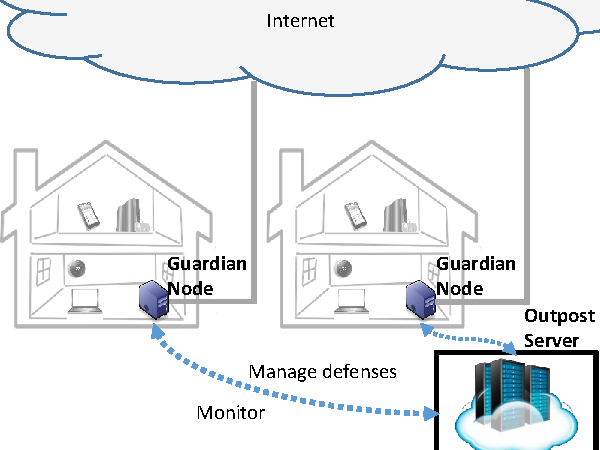
\includegraphics[width=0.95\columnwidth]{figs/highlevel.pdf}
    %\caption{\sysname architecture.}
    %\label{fig:arch}
%\end{figure}
%
%


\section{System Design}

\begin{figure}
    \centering
    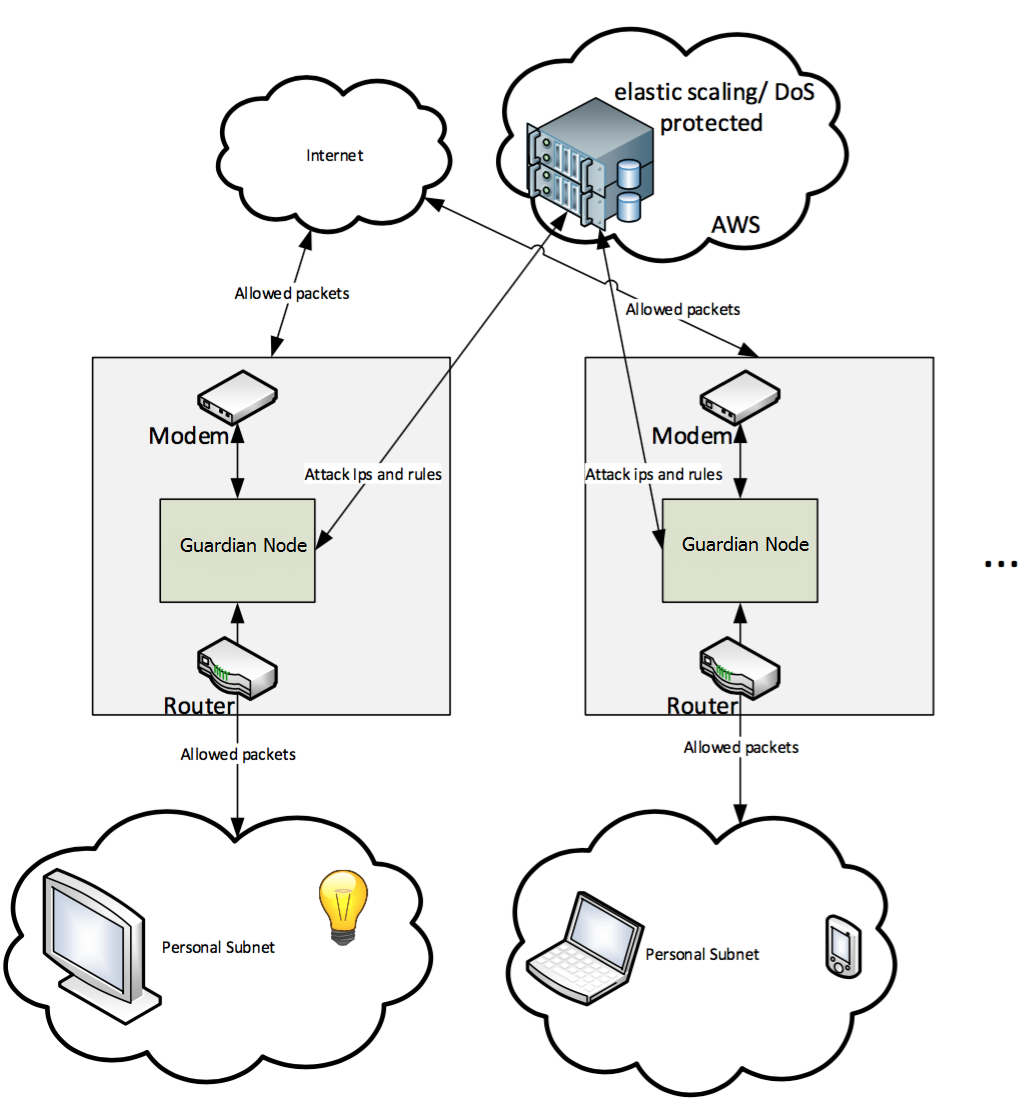
\includegraphics[height=5cm]{figs/macro.png}
    \caption{\sysname macro-level architecture}
    \label{fig:macro}
\end{figure}


\label{sec:design}

Figure\ref{fig:macro} shows the high-level design of \sysname. The keystone of the proposed architecture is the \sysname IPS device - also known as the \nodename, which must be placed in a position where it can view the entire network traffic flowing into and out of a user's network, and block all suspicious traffic. The addition of the device must be as non-intrusive as possible, requiring no modification in Modem or Router configuration. \\

Based on these factors, the ideal placement of the \nodename is between a Modem and Router. For networks using a Modem and a Router on the same device, we foresee that a production scale implementation of \sysname would place the \nodename hardware within the same box as the Modem and the Router, therefore maintaining the same architecture as shown in Figure~\ref{fig:macro}. Such \nodenames placed at the entry point of home networks can create a solid net of protection that can communicate threats as soon as they emerge. It must be noted that the responsiveness and accuracy of \sysname in deterring threats, and especially its ability to mitigate DDoS attacks, is directly proportional to the number of subnets that use this system; ideally there would be a \nodename within every household and business subnet.

\subsection{\nodename}
\label{sec:design:guardian}

\subsubsection{Hardware Design}
The BeagleBone Black, a reasonably powerful embedded device, was chosen as the \nodename since it satisfied the minimum requirements to implement the envisioned end product. The on-board 10/100 Mbps Ethernet port provided one network interface, while another interface was added using an USB to 10/100 Mbps Ethernet adapter. This prototype is deemed sufficient to display the core mechanics of the \nodename. 

\subsubsection{Software Design}
\label{sec:design:software}

The software design of a \nodename is depicted in Figure~\ref{fig:guardian}. The device has a DHCP server configured so that a Router can be added behind it. It passes all traffic from one network interface to the other. The \nodename runs Snort \cite{Roesch:1999:SLI:1039834.1039864}, a powerful Intrusion Detection/Prevent tool, to monitor traffic at both interfaces. A set of Snort rules are configured to block any suspicious traffic that satisfies any of the rules. Snort can perform protocol analysis, content searching/matching, and can be used to detect a variety of attacks and probes, such as buffer overflow, stealth port scans, CGI attacks, SMB probes, OS fingerprinting attempts, and many more. It also provides a black-list and white-list functionality that can be used to conditionally block and unblock malicious IP addresses. Snort was chosen as the IPS due to its large amount of documentation, open source software and up-to-date rule-lists, and its high regard in security communities. \\

Communication of malware alerts between various \nodenames is a key aspect of \sysname. This communication is done on a periodic basis by a set of three cron jobs running on the \nodename. These cron jobs do the following:

\begin{itemize}
    \item Keep Snort's general rules up-to-date by pulling rules and IPs from rule repositories.
    \item Push this particular guardian node's suspicious traffic to the \servname and also to pull new rules and blocked IPs from the \servname.
    \item Check for DDoS server beacons and generate new anti-DDoS rules if necessary.
\end{itemize}

The first cron job runs periodically and reads a log created by Snort that contains IP address of sources that have sent bad traffic. It then parses the source IP addresses present in the log, and updates the same to the database on the \servname (described in the following section). \\

\begin{figure}
    \centering
    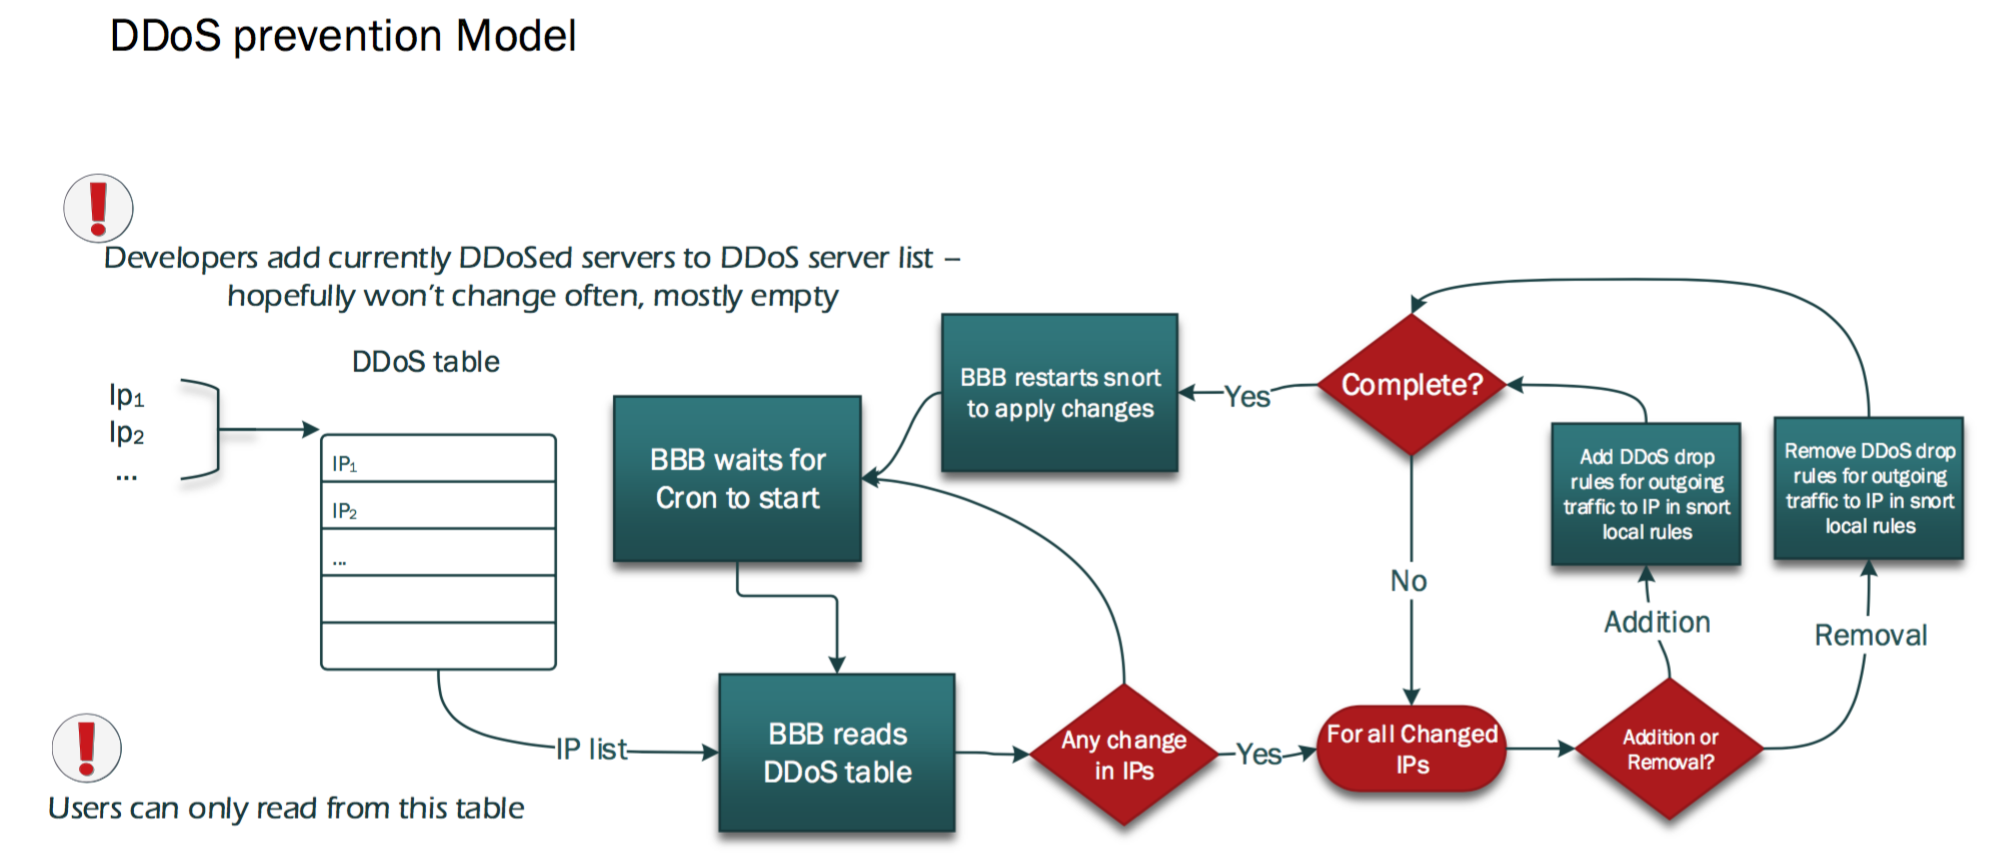
\includegraphics[width=0.95\linewidth]{figs/ddostable.png}
    \caption{Outbound DDoS prevention Algorithm}
    \label{fig:ddostable}
\end{figure}

\begin{figure}
    \centering
    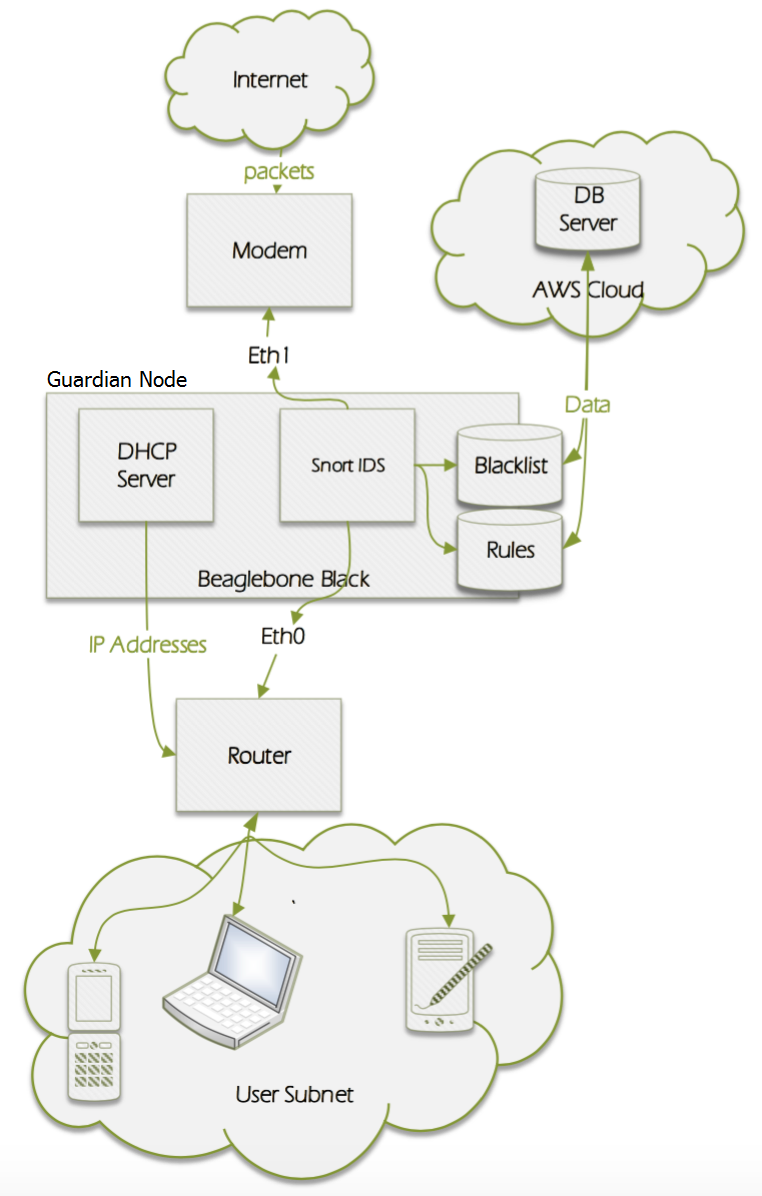
\includegraphics[width=5cm, height=6cm]{figs/guardiannode.png}
    \caption{Anatomy of a \servname}
    \label{fig:guardian}
\end{figure}

A second cron job runs periodically to fetch information from a DDoS watch list available on the \servname described below as part of the Outgoing DDoS prevention mechanism (server-side is described in Section \ref{sec:design:serverddos}). If the database provides new IP addresses (for which rules do not exist on the \nodename yet) that are currently being DDoSed, the cron job creates and adds Snort rules to drop all such outgoing DDoS traffic, thus clipping off the attack at the compromised source itself. 
This algorithm is depicted in Figure ~\ref{fig:ddostable}; Such a mechanism, when repeated over all \servnames, can prevent a DDoS attack such as the DYN DDoS attack. \\

Finally, the third cron job runs once every day at some random time and fetches the latest bad IP list from the \servname and adds it to the Snort IP Blacklist. It also fetches Snort rules from Emerging Threats ~\cite{emerging} to defend against new and emerging attack patterns. These three cron jobs, combined with Snort running on all \nodenames, together establish a system of protection that learns, communicates, and has the capacity to prevent most malware attacks.

\subsection{\servname}
\label{sec:design:server}

% TODO I know I need to crop this
\begin{figure}
    \centering
    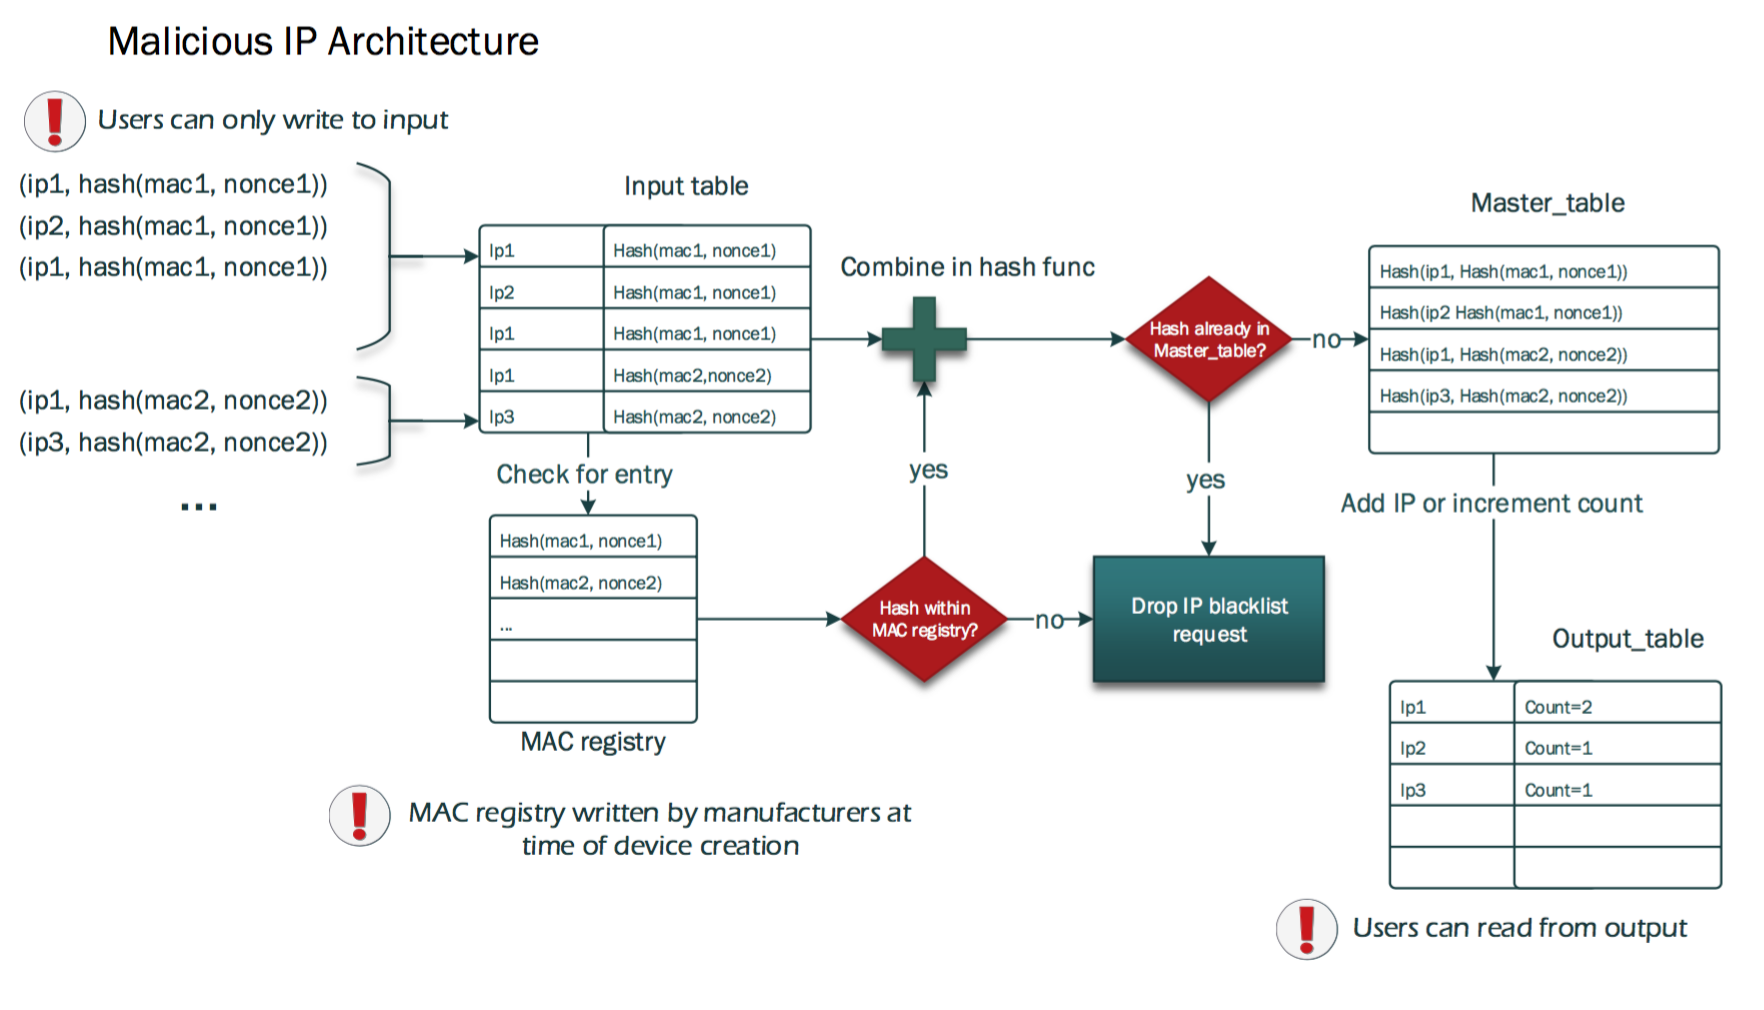
\includegraphics[width=0.95\linewidth]{figs/blacklistserver.png}
    \caption{\servname push and pull architecture}
    \label{fig:blacklistserver}
\end{figure}

The \servname is the source of intelligence for the \nodenames that it services. This server runs a database and a couple of cron job timed events to process the information within its database. This server uses its database tables to aggregate threats presented by all collected guardian nodes, process them to determine valid threats, and then present them for individual guardian nodes to read and process. As this server is an obvious line of attack for one who would wish to halt the \sysname service, it is foreseen that the server will be elastically-scaling and secure in a production level implementation. 

\subsubsection{Attack Models}
\label{sec:design:attacks}
We assume that a user will not attempt to attack or compromise the availability or function own \nodename since our system aims to protect users who are unaware that their devices have been compromised. Furthermore, the \nodename itself can be fortified from external attacks through a hardened OS image and security best practices. This leaves a malicious user two possible vectors of attack for causing harm to a particular user- either attempting to get harmful traffic through the \nodename, or else reverse-engineering the \nodename to attack the \servname itself. 
We designed the functionality of the \servname while keeping the following attack models in mind:

\begin{enumerate}
\item A malicious user may attempt to add useful IPs to the blacklist to block them for users
\item A malicious user may attempt to remove blacklisted IPs from the blacklist
\item A malicious user may attempt to read user data from the list
\end{enumerate}

\subsubsection{Server Blacklist architecture}
\label{sec:design:blacklist}
When any guardian node is created, a SHA256 hash of the node's MAC address and a random nonce stored on the \nodename's memory is entered into the mac_addr_registry table, as shown in Figure ~\ref{fig:blacklistserver}. This hash value will serve as a key for writes, to ensure that writes can only be initiated from a valid \nodename.

The \nodename is only allowed write permission to the IPv4_input table and read permission from the IPv4_output table and DDoS_output table. This policy prevents attack models 1, 2, and 3 and ensures that even if a malicious user were to reverse-engineer the device to discover a means to contact the \servname directly, the amount of damage they could cause is minor. When a \nodename is scheduled to push suspicious traffic to the \servname, it is allowed to write only into the IPv4_input table. It will write the following pair to the input table: \[\{ip_{suspicious}, SHA256(int(MAC addr), nonce)\}\] 

The \servname will process the input table to recalculate new threats at a certain frequency, and then drop the current input table. For each entry in the input table, the server first checks the SHA256 passed by the \nodename to ensure that this key is already within the mac_addr_registry. The entries that do not have a valid SHA256 hash are dropped, leaving only the valid requests. For all valid requests, a second SHA256 hash is computed, this time a hash of both the previous SHA256 result and now also the IP address declared as suspicious \[SHA256(\{ip_{suspicious}, SHA256(int(MAC addr), nonce)\}) \]. The \servname checks whether this hash is already in the IPv4_master_list server, which is a list of the SHA256, IP combinations that have previously been entered- if this is a new suspicious IP, or it is a known suspicious IP being reported by a new and valid \nodename, it will be pushed to the IPv4_output table. This second hash function ensures that a given \servname receives only one vote towards a given IP address, as a means to prevent against attack model 1. 

If this IP is a new entry, it will be entered into the table with a count of 1; if it already exists within the table, its count will be incremented. Once the count tallied against the IP reaches a sufficiently high number proportional to the number of reported threats, the IP will be pushed as output to requesting \nodenames, and blocked automatically by all \nodenames. Relying on a count before pushing a suspicious IP also helps prevent attack model 1 from occurring. 

\subsubsection{Server Outgoing DDoS prevention}
\label{sec:design:serverddos}

As mentioned above in Section ~\ref{sec:design:software}, the \servname also provides a method to prevent outgoing DDoS traffic from a \nodename's subnet out to a DDoS target. This system is much more simple than the blacklist method described above: in this case, the DDoS victim list will be edited by \sysname administrators, and only reading will be allowed for all \nodenames. \sysname administrators will confirm the existence of a DDoS attack through an alternate channel, possibly a third party DDoS \cite{DDoSPreventionTools} working with \sysname administrators, and then add the relevant IPs or CIDR ranges to the IPv4_ddos table. \nodenames will use the cron described above to add and remove rules to prevent outgoing DDoS attacks.
\section{Evaluation and Performance}
\label{sec:eval}

We evaluated CommunityGuard by both the effectiveness of its intended operation~\ref{sec:eval:operation} as well as by network performance while the system was running in-line ~\ref{sec:eval:performance}.  


\subsection{Operation}
\label{sec:eval:operation}

To test the effectiveness of the system, we evaluated two core capabilities of CommunityGuard which are described below.
Our \textit{Test Setup} includes two Guardian Nodes present on different networks, which were used to test the system to check if blacklisted IP addresses updated by one Guardian Node  was communicated to the other. Both Guardian Nodes connected to the Community Outpost server with the same periodicity.

%\begin{figure}
%    \centering
%    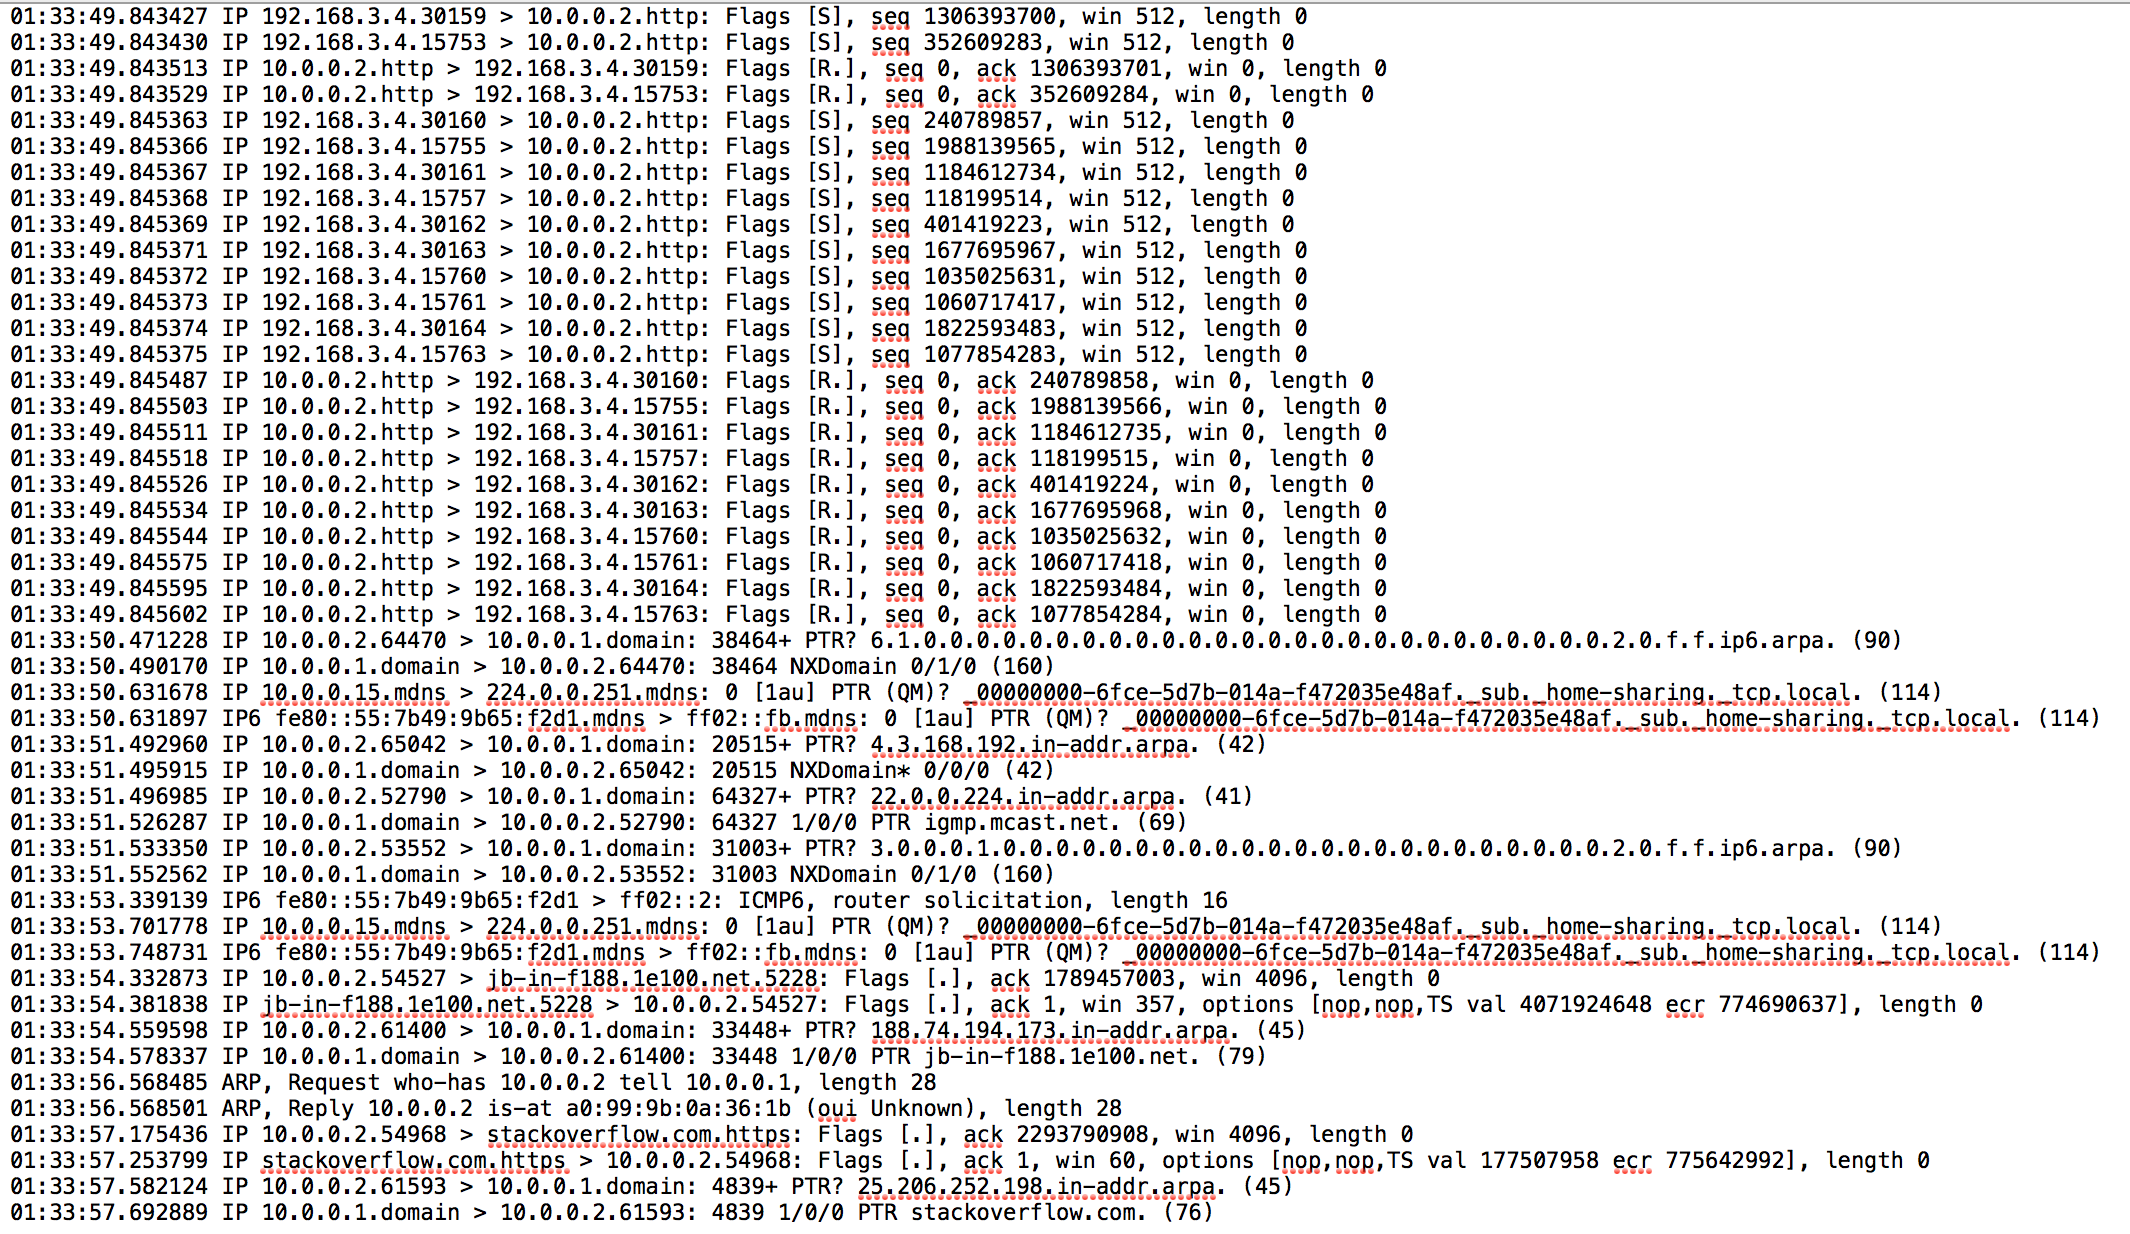
\includegraphics[width=0.95\linewidth, height=4cm]{figs/tcpdump.png}
%    \caption{TCP dump at DDoS target}
%    \label{fig:tcpdump}
%\end{figure}
\subsubsection{Prevent and log incoming malicious traffic}
\label{sec:eval:preventout}

 Snort rules were configured to block IP traffic that contained malicious content. There are thousands of open-source snort rules available that can alert and drop malicious traffic like worms, illegal attempts at accessing FTP or telnet, and a range of attacks ~\cite{Roesch:1999:SLI:1039834.1039864}. However, we did not wish to receive actual malicious traffic in testing due to infrastructure and resource restrictions. Instead, the team wrote a few snort rules to treat some arbitrary safe traffic as malicious and configured rules to drop such traffic. 
%Figure~\ref{fig:snortrule} shows a screenshot of a sample Snort rule that alerts and logs all traffic containing the word "cat". Figure~\ref{fig:snortrule} also shows a section of the log where the "malicious" traffic was spotted. 
The cron job (discussed in \ref{sec:design:software}) parsed the log and updated the DB about the source from where possible malicious traffic was originating. Depending on a majority of votes (this majority was artificially elevated in our test case since only two Guardian Nodes were present), the Community Outpost proceeded to conditionally add the malicious source IP to the blocked list. Newly confirmed bad IP addresses are fetched when the cron job responsible for adding blacklisted IP addresses next runs on the Guardian Nodes. %In case of the log shown in Figure \ref{fig:snortrule}, IP addresses "107.23.60.9" and "72.21.91.66" were treated as Bad IPs, and were subsequently blocked by both Guardian Nodes once the cron job refreshed the blacklist with the latest one from the Community Outpost.

\subsubsection{Prevent outbound DDoS attacks}
\label{sec:eval:outddos}

This was tested by adding "fake" DDoSed IP addresses to the DDoS watch list on the Community Outpost. The DDoSed IP addresses were friend machines in another network. In a real world implementation, we assume that a Third Party DDoS protection service \cite{DDoSPreventionTools} that has been specifically employed for the job would update the DDoSed IP addresses to the CommunityGuard administrators. The team added the DDoSed IP addresses manually in order to test this functionality. A TCP SYN DoS attack was simulated with hping3 \cite{hpingReferralPaper} \cite{hping}.  The cron job that was checking for new updates from the database fetched these IP addresses every minute and checked for a match in the existing list of DDoSed IP addresses maintained at each Guardian Node. New Snort drop rules were created for these IP addresses if a match was not found. The new rules prevent all outbound DDoS traffic to the IP addresses fetched from the DDoS watch list. 

An important point to note here is that the network was still allowed to send legitimate traffic to these attacked IP addresses because Snort rules were configured to monitor the pattern of a DDoS attack before dropping that traffic. One such Snort rule is shown in Figure ~\ref{fig:snortrule1} which detects an outgoing SYN flood attack from the home network to an external network. Figure ~\ref{fig:snortrule1} also shows the log created by Snort when it detects and drops an outgoing DDoS attack as soon as the cron job fetches the DDoS watch list from the Community Outpost. The Snort rule detects TCP-SYN DDoS attack patterns and drops all such outgoing traffic. However, benign TCP traffic is still allowed to pass through. This was tested using the netcat tool \cite{netcat} to communicate between the attacking system and the attacked system via TCP while Snort was actively blocking all outgoing TCP-SYN DDoS attacks to the target IP.

\subsection{Performance}
\label{sec:eval:performance}
\subsubsection{Load test}
\label{sec:eval:loadtest}
The Guardian Node is designed to be inserted in-line somewhere before the Router, which implies that the Guardian Node could be introducing a possible bottleneck and stalling traffic coming into and going out of the personal network. Therefore, it was necessary to verify the performance of the Guardian Node while it was fully functional. Speed tests were taken at intervals of 5 minutes under light, average and heavy load conditions to conform performance compliance. Light load was simulated by opening 1-3 video Live streams, a few browsers with medium flash content, one active upload and few Social media pages over 6 different devices ranging from desktops to tablets and mobile phones. Average load was simulated by opening 3-5 live streams, 4-6 pages with high flash content and 2-3 active uploads distributed over the same set of devices. Heavy load was simulated by increasing to 6-8 live streams, 8-10 pages with high flash content and 4-5 active uploads distributed over the same set of devices. Figure ~\ref{fig:graph} shows the performance represented as a linear plot. As can be seen, the performance data is very similar between the baseline and the test case. On an average the test case appears to be slightly lower than the baseline case which can be significantly attributed to the following hardware deficiencies.
\begin{itemize}
    \item USB to 10/100 Mbps Ethernet adapter --
    The Guardian Node hardware, which in this case was a BeagleBone Black, has only one on-board 10/100 Mbps Ethernet port. An USB to 10/100 Mbps Ethernet adapter was added since the Guardian Node required two network interfaces. Speed of transfer was therefore severely limited by the speed of conversion.
    \item Slow SD card writes --
    The Guardian Node was running a Linux Operating System that was mounted on a SD card. Transfer speeds were also affected by comparatively slow SD card write times.
\end{itemize}

%\begin{figure}
%    \centering
%    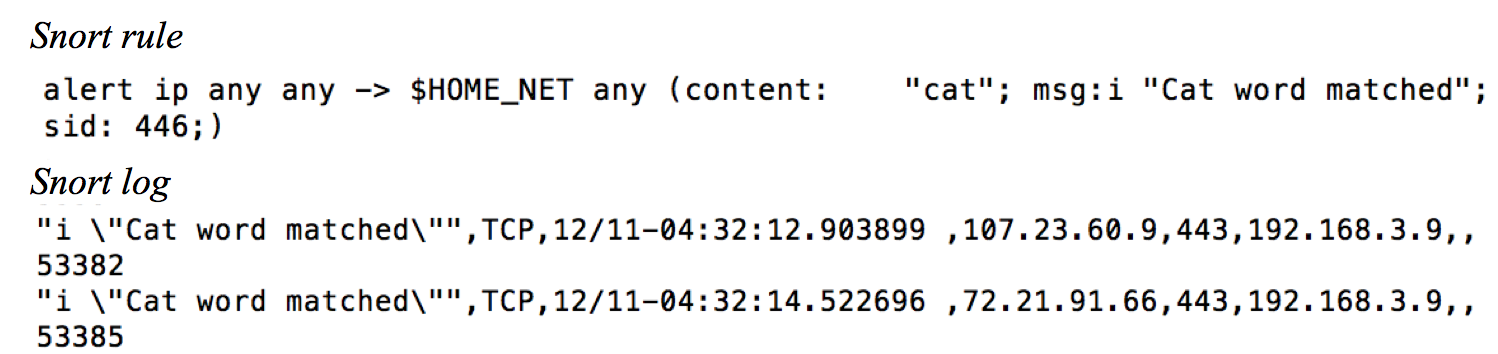
\includegraphics[width=0.95\linewidth]{figs/catrule.png}
%    \caption{Sample Snort rule and log}
%    \label{fig:snortrule}
%\end{figure}

\begin{figure}
	\centering
%	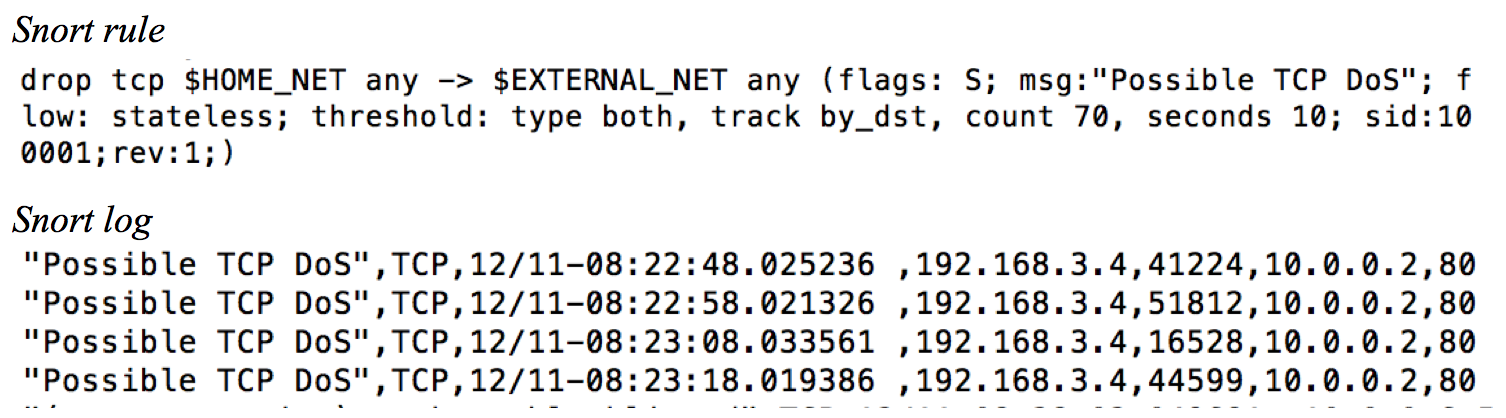
\includegraphics[ height=2.2cm]{figs/ddosrule.png}
	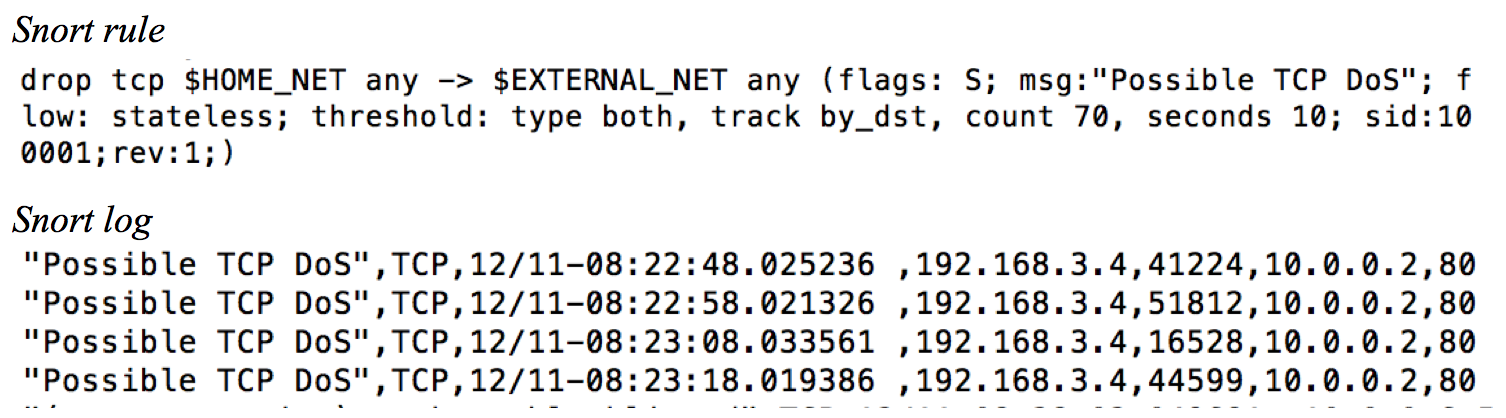
\includegraphics[width=\columnwidth]{figs/ddosrule.png}
	\caption{Sample Snort DDoS prevention rule and log}
	\label{fig:snortrule1}
\end{figure}

\begin{figure*}
	\centering
%	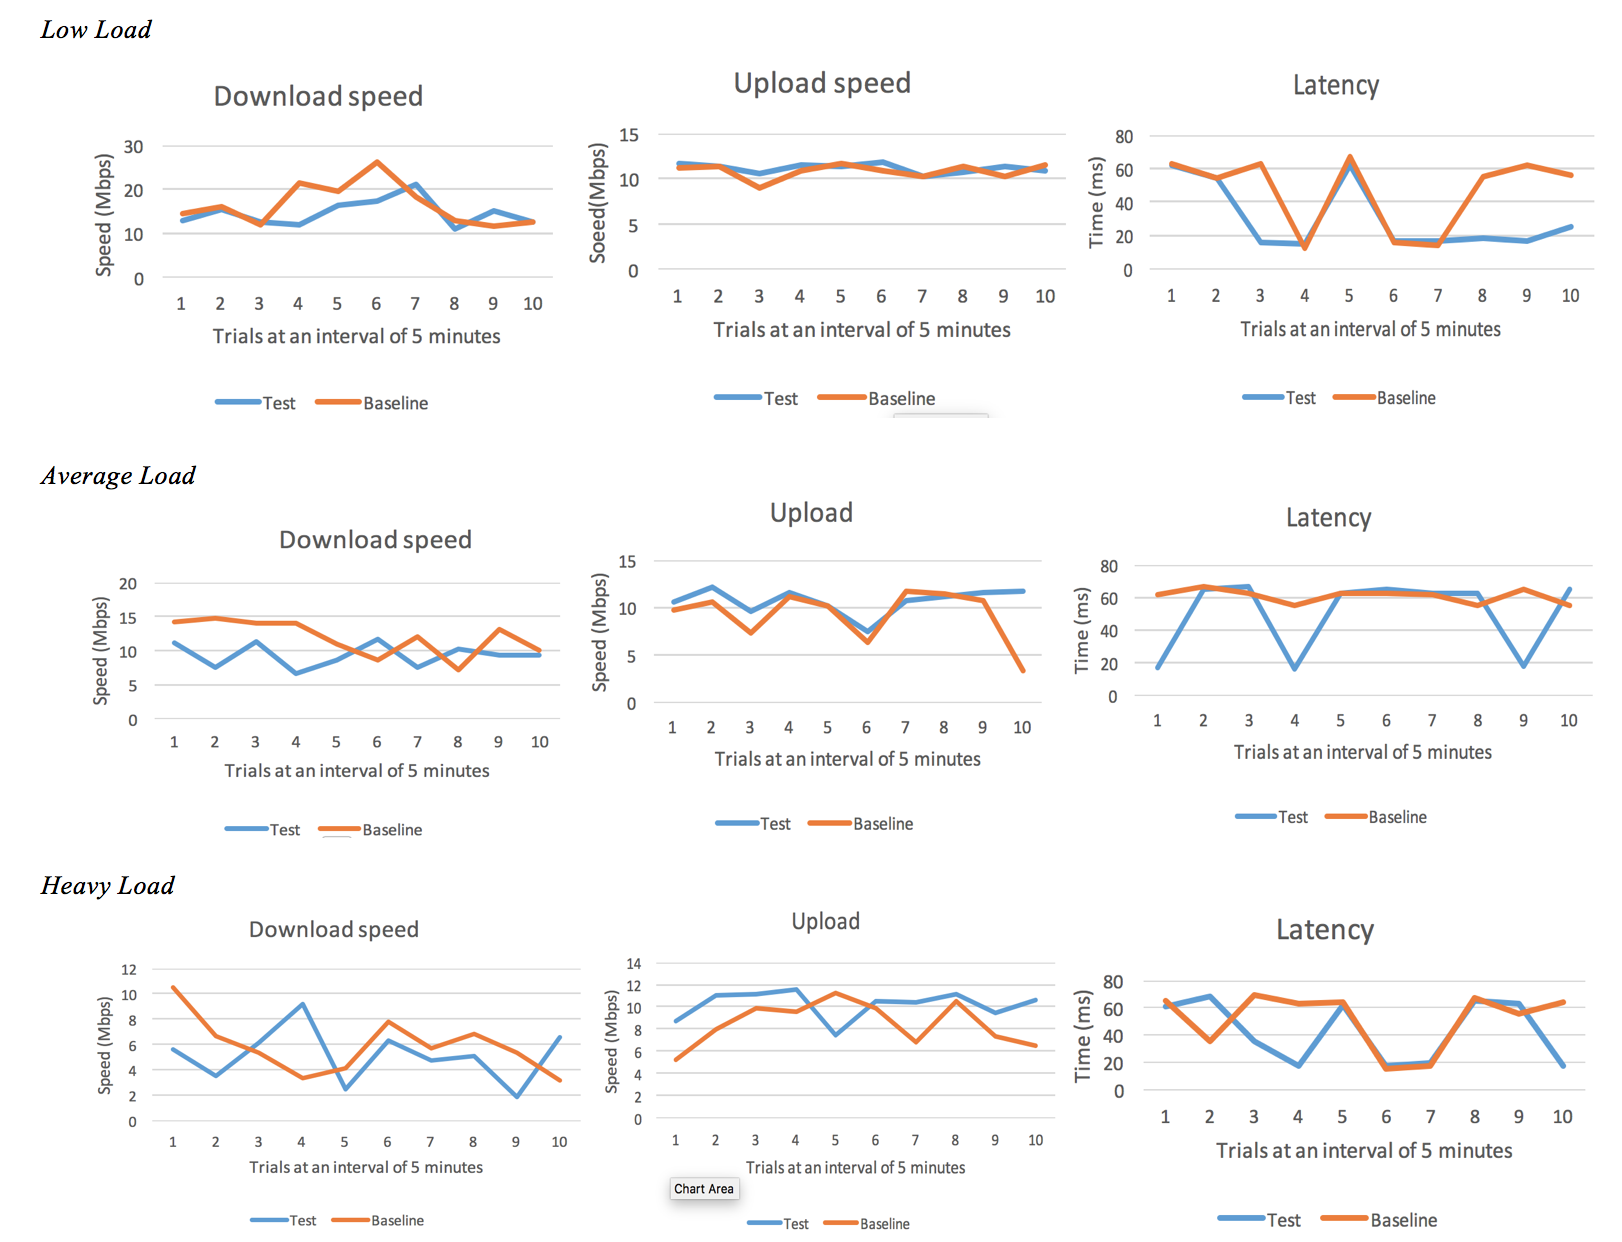
\includegraphics[width=0.7\linewidth, height=5.5cm]{figs/graph.png}
	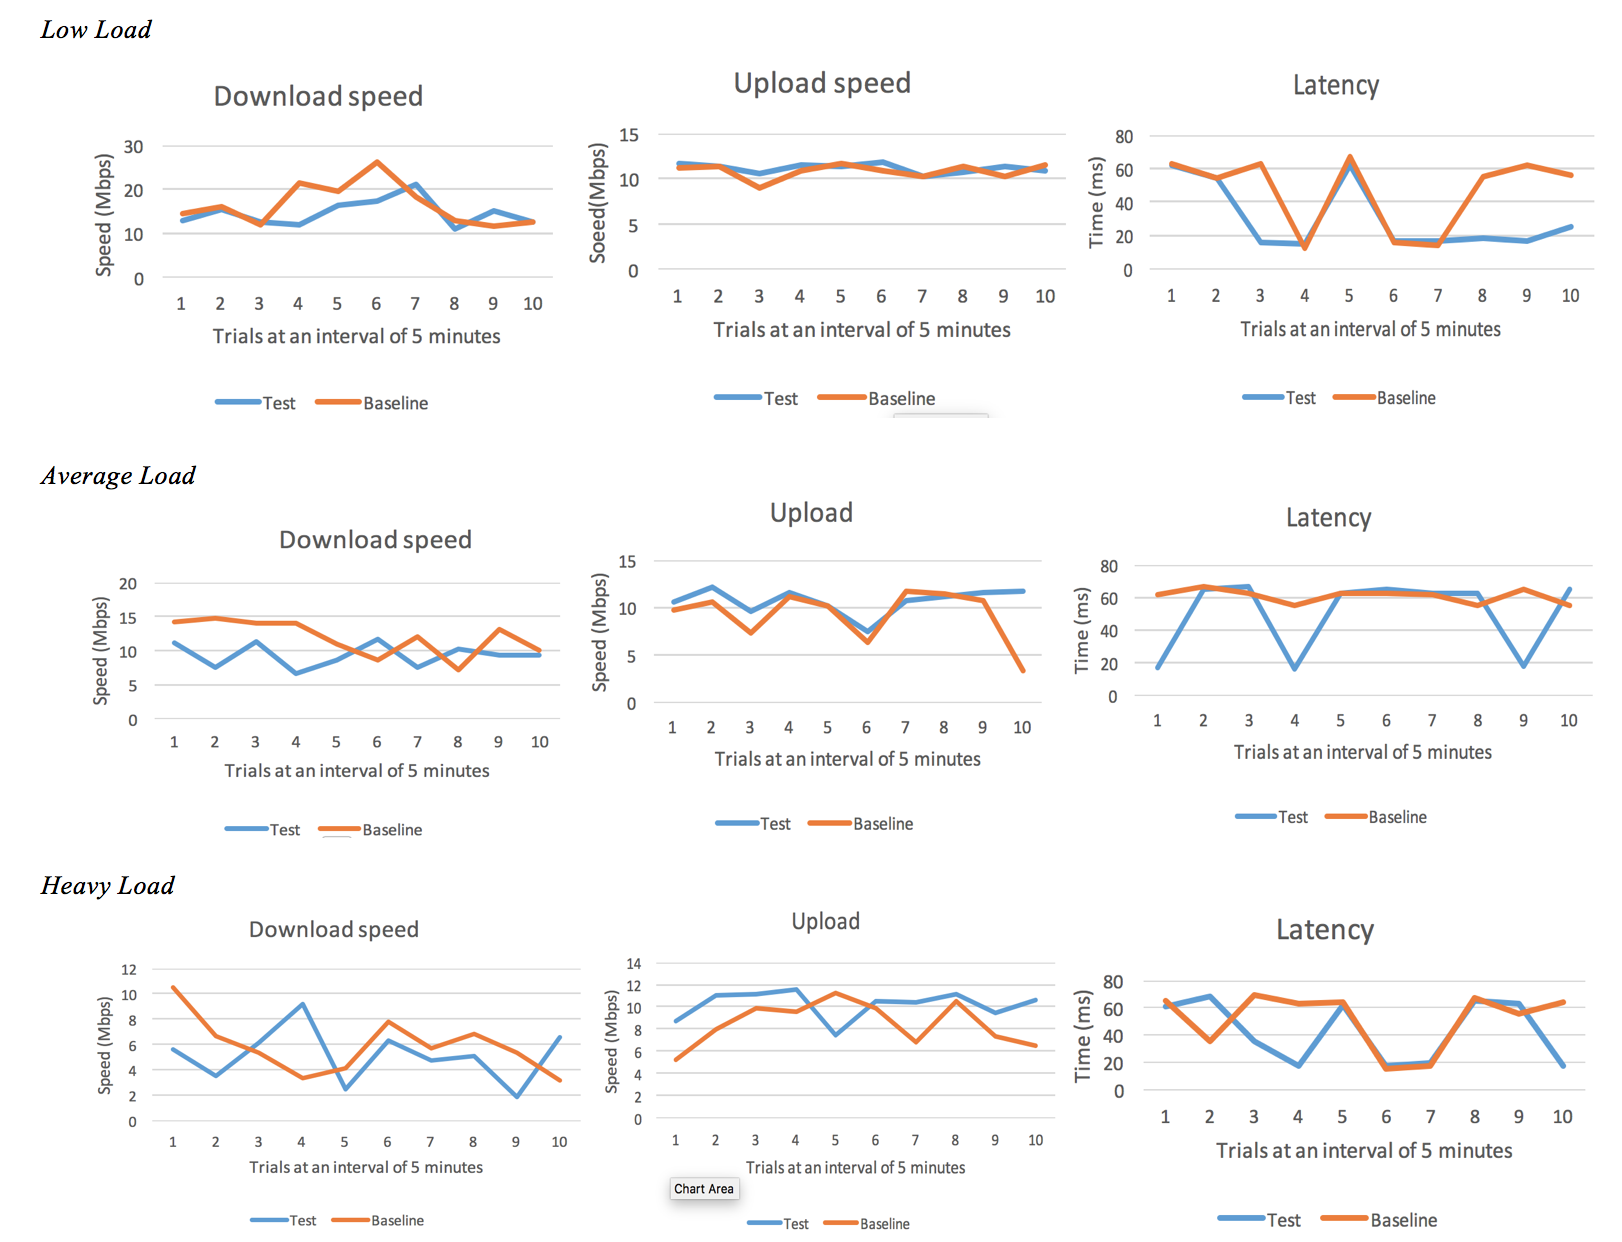
\includegraphics[width=0.75\linewidth]{figs/graph.png}
	\caption{Results of Snort throughput tests: test=CommunityGuard, baseline=no CommunityGuard}
	\label{fig:graph}
\end{figure*}

\subsubsection{Performance vs. number of Snort rules}
\label{}
Snort provides the freedom to configure as few rules or as many rules as required. The Load Test mentioned in Section \ref{sec:eval:loadtest} was done with approximately 7000 Snort rules configured and functioning. Speed tests were also conducted for a number of rules ranging between 100 to 10000. It was seen that the number of rules did not affect speed test results as much as one would expect. Speed measurements indicated similar values to those shown in Figure ~\ref{fig:graph}. This was attributed to the fact that Snort processes utilized around 150 to 200 MB of RAM in all cases ranging between 100 to 10000 rules. Figure ~\ref{fig:ramutil} shows the RAM utilization without Snort running, Snort running with 156 rules and Snort running with 9863 rules. 

The CommunityGuard team  feels that the set of running Snort rules can be further optimized for better processor and RAM utilization. Optimization of Snort rules will be pursued as future work. It is to be noted that increasing traffic from 100 Mbps to 400 Mbps will increase the RAM requirement to almost 1GB for 100-10000 rules. The implementation of Snort on the Guardian Node was using much less RAM since network traffic was limited to 100 Mbps by the Ethernet card. Dealing with higher traffic speeds would require specialized hardware. In an ideal implementation, the Guardian Node would have a network card with performance specifications equivalent to it's router's network card.

\begin{figure}
    \centering
%    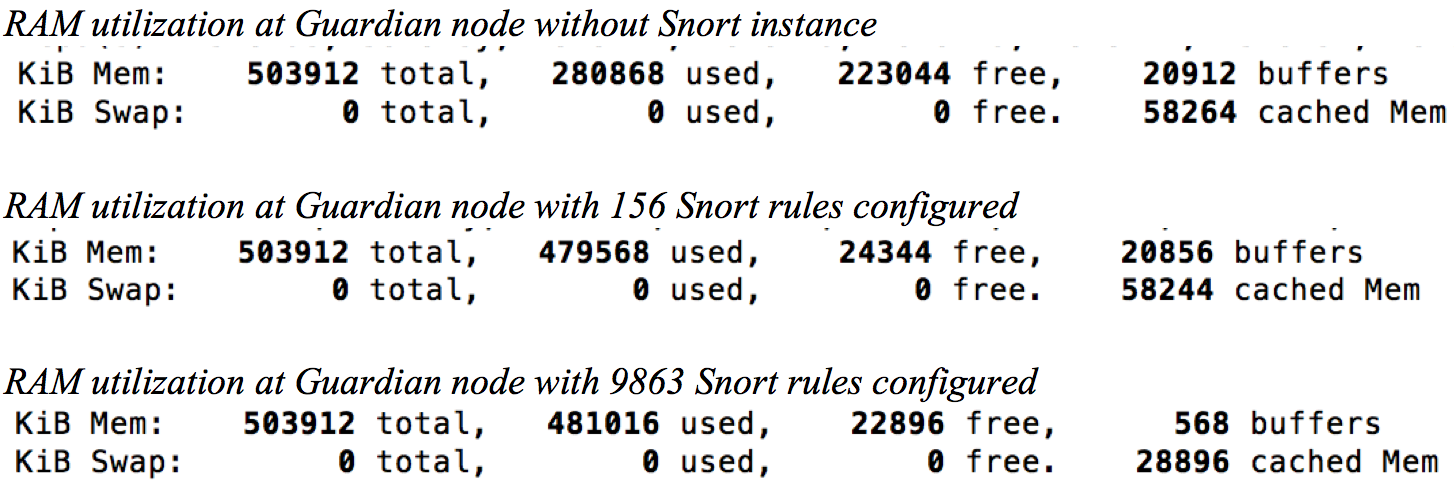
\includegraphics[width=0.85\linewidth,  height=2cm]{figs/SnortRam.png}
    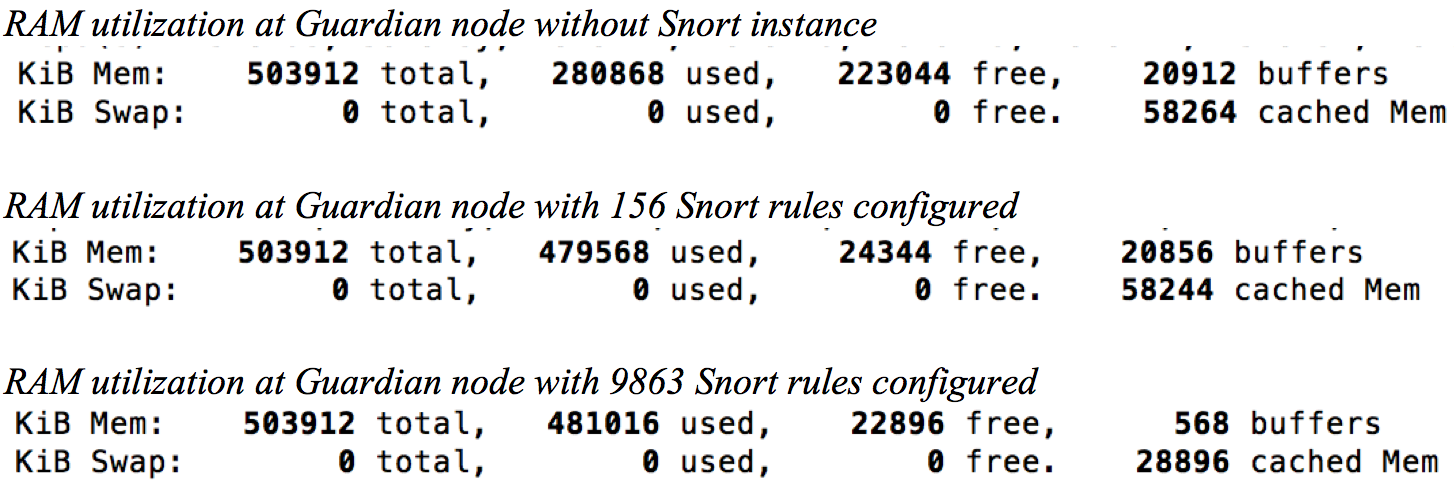
\includegraphics[width=0.85\columnwidth]{figs/SnortRam.png}
    \caption{RAM Utilization on the Guardian Node}
    \label{fig:ramutil}
\end{figure}


\vspace{0.1in}
\section{Related Work}
\label{sec:related}

Collaborative Network Security is not a new topic, and some previous work has been done in this domain. Chen,  Dong et al. \cite {collaborative} describe a collaborative security for multi-tenant data centers using a security center. Mu, Chen, et al. \cite {metro} propose a collaborative security management system for Metropolitan Area Networks using a P2P network. Both papers do not address security for a common user's local network or large scale vulnerabilities introduced by personal devices that have weak security such as IoT devices. Also, both papers do not address situations where a malicious user might try to block valid traffic for all peers by sending bad data to the central security system, nor do they deal with preventing an outbound DDoS attack. These are aspects we have dealt with in our paper. Mirkovi´c, Prier et al. \cite{attackddos} have talked about preventing a DDoS attack at the source by monitoring 2-way traffic periodically and at all points of time. They do not talk about cloud sourcing this information to prevent similar outbound DDoS attacks on all networks and mostly focus on detecting DDoS attacks based on the pattern. As far as DDoS attacks are concerned, we mostly focus on the cloud sourcing aspect of preventing a large scale DDoS attack.
\section{Conclusions and Future Work}
\label{sec:concl}

%\subsection{Conclusion}
%\label{sec:concl:main}
As network security will only become more crucial over time, we aspire to a future where users' personal area networks and devices defend themselves and each other from emerging threats. To this end, we introduced the design, prototype, and evaluation of CommunityGuard, an in-line home cyber-security system where a Guardian Node in each home shares new threats with nodes in other homes. This provides a sort of herd immunity against new attacks. As soon as an attack claims a victim, all of the victim's peers will be informed, and will repel the same attack against their own subnets. 

%We introduce a high-level architecture for the entire system, as well as an initial prototype of both the Guardian Nodes the Community Outpost. We consider some potential attack vectors against the server and show how the design of the server mitigates such attacks.  

%To demonstrate the novelty and benefits of CommunityGuard, we implemented a very small scale version of the architecture. We used two BeagleBone Black embedded systems to each host a Guardian Node and created an CommunityGuard using a medium-class Amazon Web Services EC2 instance. Using this minimum-viable model, we configured and implemented the necessary software on each device, and then used this setup to test the architecture and the performance of the CommunityGuard system. Through this implementation, we were able to do the following:
%
%\begin{itemize}
    %\item Create the Community Outpost server tables and input processing.
    %\item Describe and address several potential attack models against the Community Outpost server design through its architecture and security permissions.
    %\item Demonstrate alerting and blocking traffic using the Guardian Node, as well as push to/pull from the Community Outpost server.
    %\item Demonstrate that using the prototype Guardian Node with sub-optimal hardware had a low impact on a user's internet browsing performance, and that there is much room for improvement in this area.
%\end{itemize}
%
%\subsection{Further Work}
%\label{sec:concl:further}

As this is only a first step toward our overall vision, we envision much future work.
This includes large scale testing (deploying in many homes), exploration of alternate hardware platforms, integration into routers, expanding on the correlation across anomalies seen in various Guardian Nodes, mathematically determining optimal thresholds for IP blacklisting, and exploring 
monitoring and defense mechanisms beyond snort, such as deploying specific DDoS scrubbing network functions (as was done in Bohatei~\cite{bohatei} for ISP networks).

%We have tested this system on a very small scale utilizing two BeagleBone Black devices communicating to one AWS server- we can think of several areas of further development for CommunityGuard, including the following:
%
%(i) Creating a very large-scale implementation ( \textgreater 10,000 Guardian Nodes) and testing its performance and security.
%(ii) Breaking up Community Outpost servers into regions and/or caching the blacklist so as to bound its growth.
%(iii) Incorporating Guardian Node processing into a router rather than an additional device.
%(iv) Re-implementing and performance-testing the Guardian Node with more specialized hardware.
%(v) Optimizing the Snort configuration and rules to fit the right hardware and threat model.
%(vi) Running multiple Snort instances in a multi-core device to prevent downtime while Snort rules reload.
%(vii) Exploring monitoring and defense mechanisms beyond snort, such as deploying specific DDoS scrubbing network functions (as was done in Bohatei~\cite{bohatei} for ISP networks).
%
%\begin{enumerate}
%\item Creating a very large-scale implementation ( \textgreater 10,000 Guardian Nodes) and testing its performance and security
%\item Breaking up Community Outpost servers into regions and/or caching the blacklist so as to bound its growth
%\item Incorporating Guardian Node processing into a router rather than an additional device
%\item Re-implementing and performance-testing the Guardian Node with more specialized hardware
%\item Optimizing the Snort configuration and rules to fit the right hardware and threat model
%\item Running multiple Snort instances in a multi-core device to prevent downtime while Snort rules reload
%\end{enumerate}

%Some such area There remains design work to be done on the scaling of the project as we believe that the benefit of this system scales proportionally to the proportion of subnets utilizing CommunityGuard. It is still left to be determined whether there would be only one Community Outpost server or perhaps several Community Outpost servers separated by region, and it is unknown how such a design would affect the performance and security of the CommunityGuard system. \\

%Another great follow-up to this project would be to re-implement the project with a more specialized hardware, or perhaps even to investigate running a Guardian Node as code on a router itself. We believe that the performance issues that result from running an in-line Guardian Node would be alleviated with the introduction of a more specialized hardware device. \\

%As the number of Guardian Nodes and the number of reported threats would rise over time, the list of threats within the Community Outpost might become quite unmanageable. To solve this problem, we imagine a sort of caching on threats based on frequency and geographical prevalence of attacks. Additionally, a few levels of threat caching would improve performance while still keeping the Guardian Node current and robust to attacks. \\

%Finally- the set of rules used by Snort are not run-time configurable as it stands, but there are ways to achieve this such as running two instances of Snort simultaneously with shared memory and a multi-core processor. A future implementation with specialized software will solve this issue and keep the Guardian Node's IPS running at all times.
%\pagebreak

%\footnotesize
\bibliography{refs}
\bibliographystyle{abbrv}

\end{document}
